\section{Gantt diagram}
\label{sec:gantt}

A Gantt diagram gives the team an overall overview over the project and the time available by giving a representation of all the work hours, milestones and deadlines that is involved in a project. The diagram is divided into packets called sprints, periods of unavailability, like vacations, and milestones representing major goals or deliveries.
The Gantt diagram for our project is given in figure~\ref{fig:gantt}.


\begin{figure}[H]
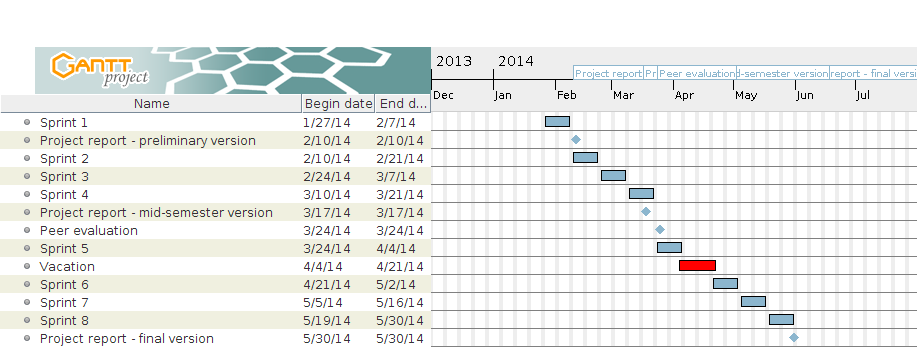
\includegraphics[width=\textwidth]{ch/planning/fig/gantt.png}
\caption{The Gantt diagram with sprints and milestones.}
\label{fig:gantt}
\end{figure}
